%%%%%%%%%%%%%%%%%%%%%%%%%%%%%%%%%%%%%%%%%%%%%%%%%%%%%%%%%%%%%%%%%%%%%%%%%%%%%%%%%%%%%%%%%%%%%%%%%%
\begin{frame}{Point de départ de l'étude}
\begin{columns}[t]
\begin{column}{7cm}
\begin{block}{On dispose de :}
\begin{itemize}
 \item Un plan initial (remplissage d'espace)
 \item Un premier métamodèle (krigeage)
\end{itemize}
\end{block}

\begin{exampleblock}{Objectif}
 Ajouter des expériences pour augmenter la qualité du métamodèle
\end{exampleblock}


\end{column}

\begin{column}{5cm}
\begin{figure}
	\centering
		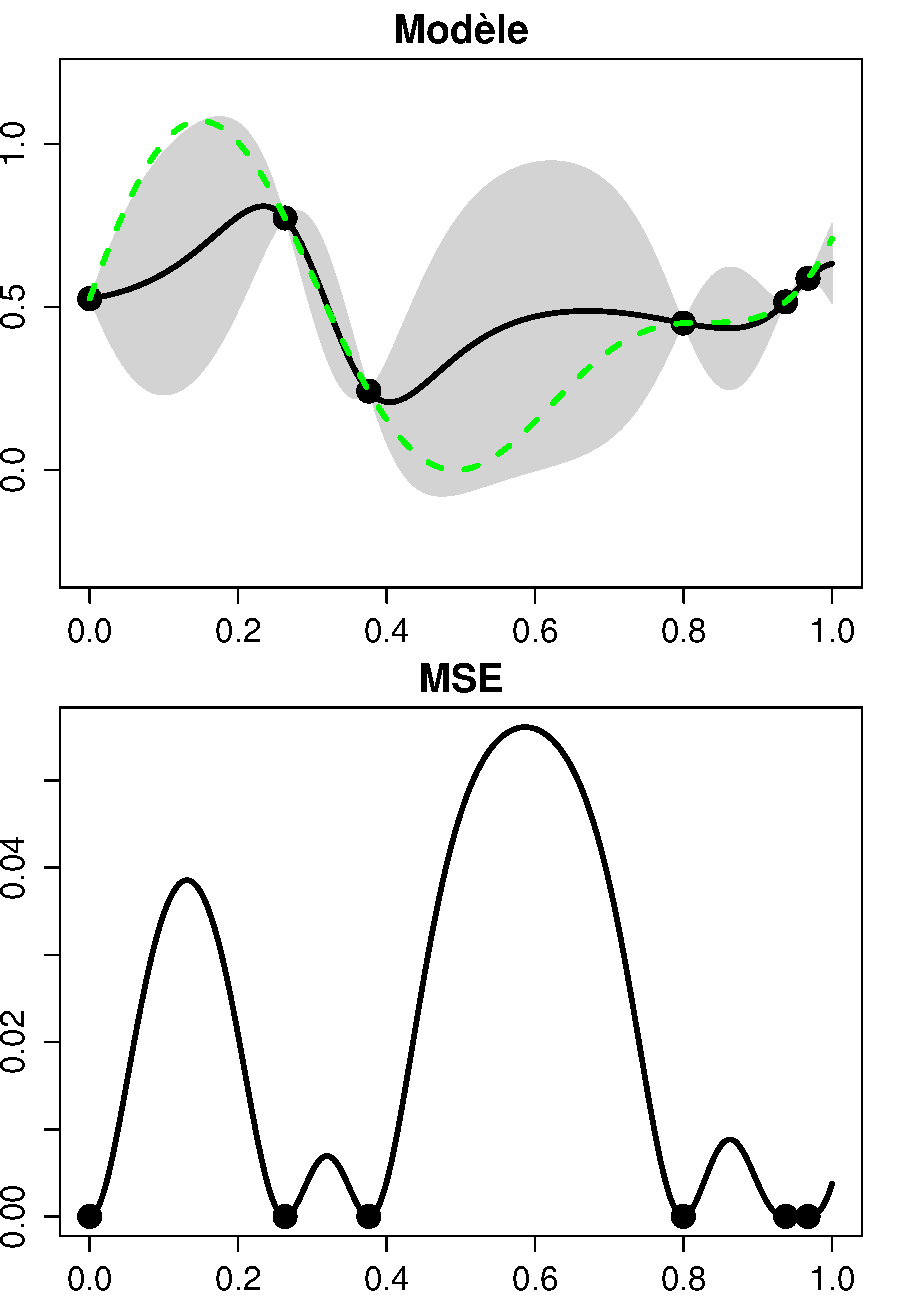
\includegraphics[trim=0 110mm 0 0, clip, width=\textwidth]{autres/MSE.pdf}
\end{figure}
\end{column}
\end{columns}
\end{frame}
%%%%%%%%%%%%%%%%%%%%%%%%%%%%%%%%%%%%%%%%%%%%%%%%%%%%%%%%%%%%%%%%%%%%%%%%%%%%%%%%%%%%%%%%%%%%%%%%%%
\begin{frame}{Peut-on s'aider du métamodèle ?}
\begin{columns}[t]
\begin{column}{6cm}
\begin{block}{Hypothèse principale}
Les paramètres de covariance sont connus avec précision.
\end{block}

\begin{block}{Mesure de la qualité du modèle} 
Variance de prédiction (MSE)
\end{block}

\begin{beamercolorbox}[sep=1em,wd=\columnwidth]{postit}
Le métamodèle indique où l'erreur de prédiction est potentiellement la plus grande !
\end{beamercolorbox}

\end{column}

\begin{column}{6cm}
\begin{figure}
	\centering
		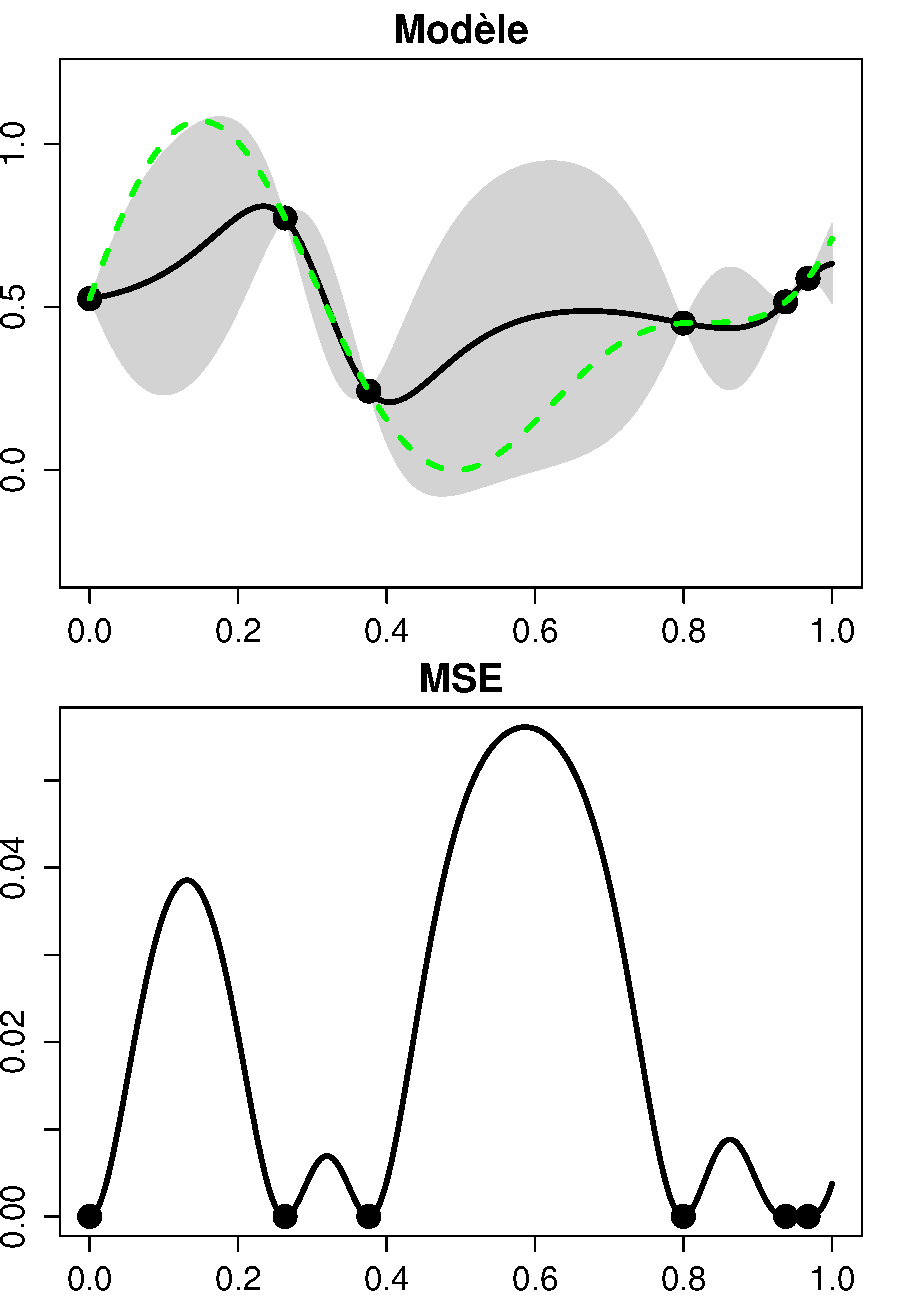
\includegraphics[width=.8\textwidth]{autres/MSE.pdf}
\end{figure}
\end{column}
\end{columns}
\end{frame}
%%%%%%%%%%%%%%%%%%%%%%%%%%%%%%%%%%%%%%%%%%%%%%%%%%%%%%%%%%%%%%%%%%%%%%%%%%%%%%%%%%%%%%%%%%%%%%%%%
\begin{frame}{Enrichissement séquentiel guidé par la variance du modèle}

\textbf{On ajoute des observations une par une en suivant le schéma :}

\begin{block}{Algorithme (boucle)}

\begin{enumerate}
	\item On cherche le point où la variance est maximum : $\mathbf{x}* = \arg \max_D MSE (\mathbf{x})$
	\item On ajoute une nouvelle observation en ce point : $\mathbf{x}_i = \mathbf{x}*$
	\item On met à jour le métamodèle (plan d'expériences et observation, + éventuellement paramètres de covariance)
\end{enumerate}
\end{block}

\begin{alertblock}{Attention !}
 La recherche de $\mathbf{x}*$ nécessite un algorithme d'optimisation.
\end{alertblock}

\end{frame}
%%%%%%%%%%%%%%%%%%%%%%%%%%%%%%%%%%%%%%%%%%%%%%%%%%%%%%%%%%%%%%%%%%%%%%%%%%%%%%%%%%%%%%%%%%%%%%%%%%
\begin{frame}{Illustration}
\begin{figure}
	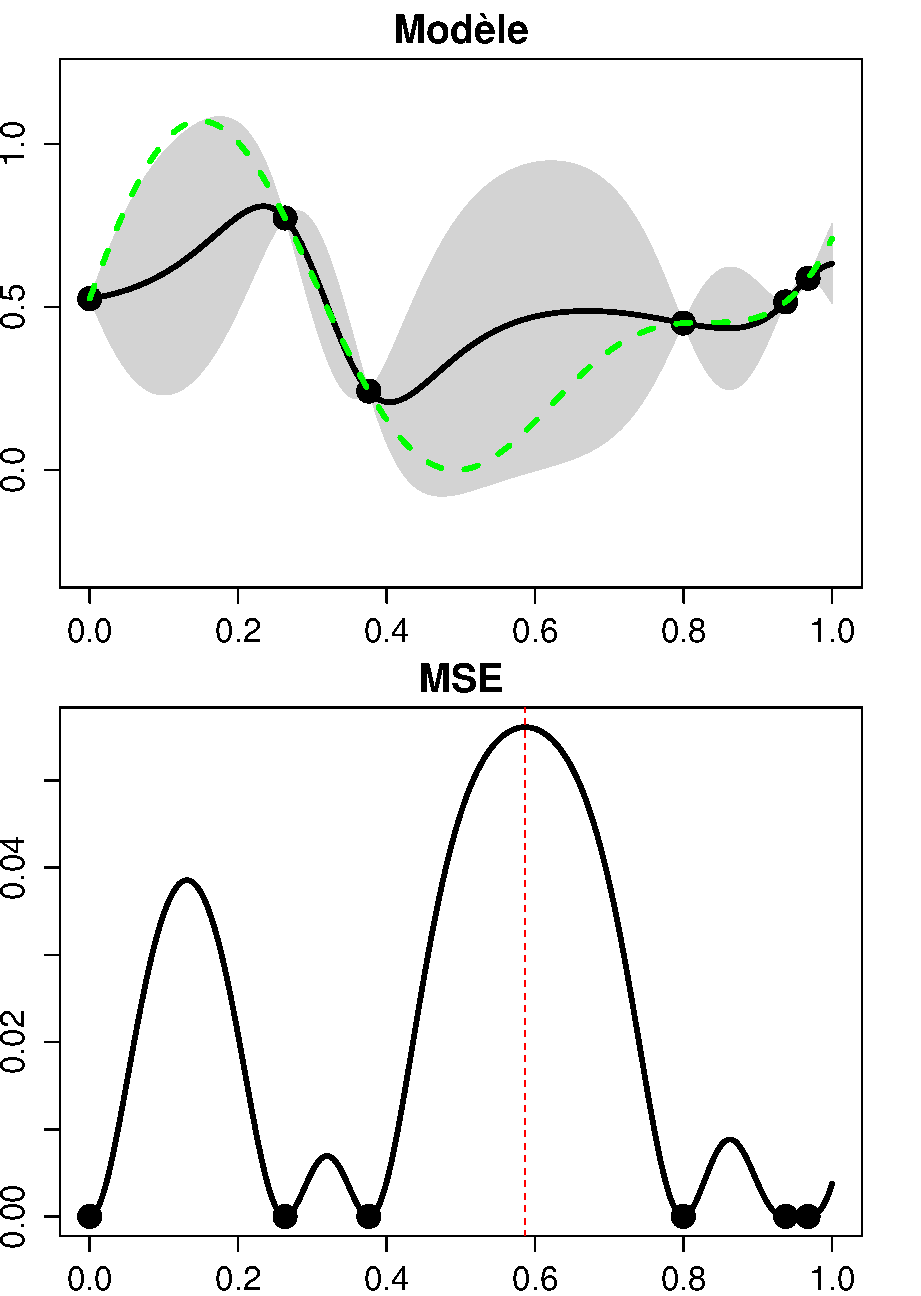
\includegraphics[width=.49\textwidth]{autres/MSE2.pdf}
	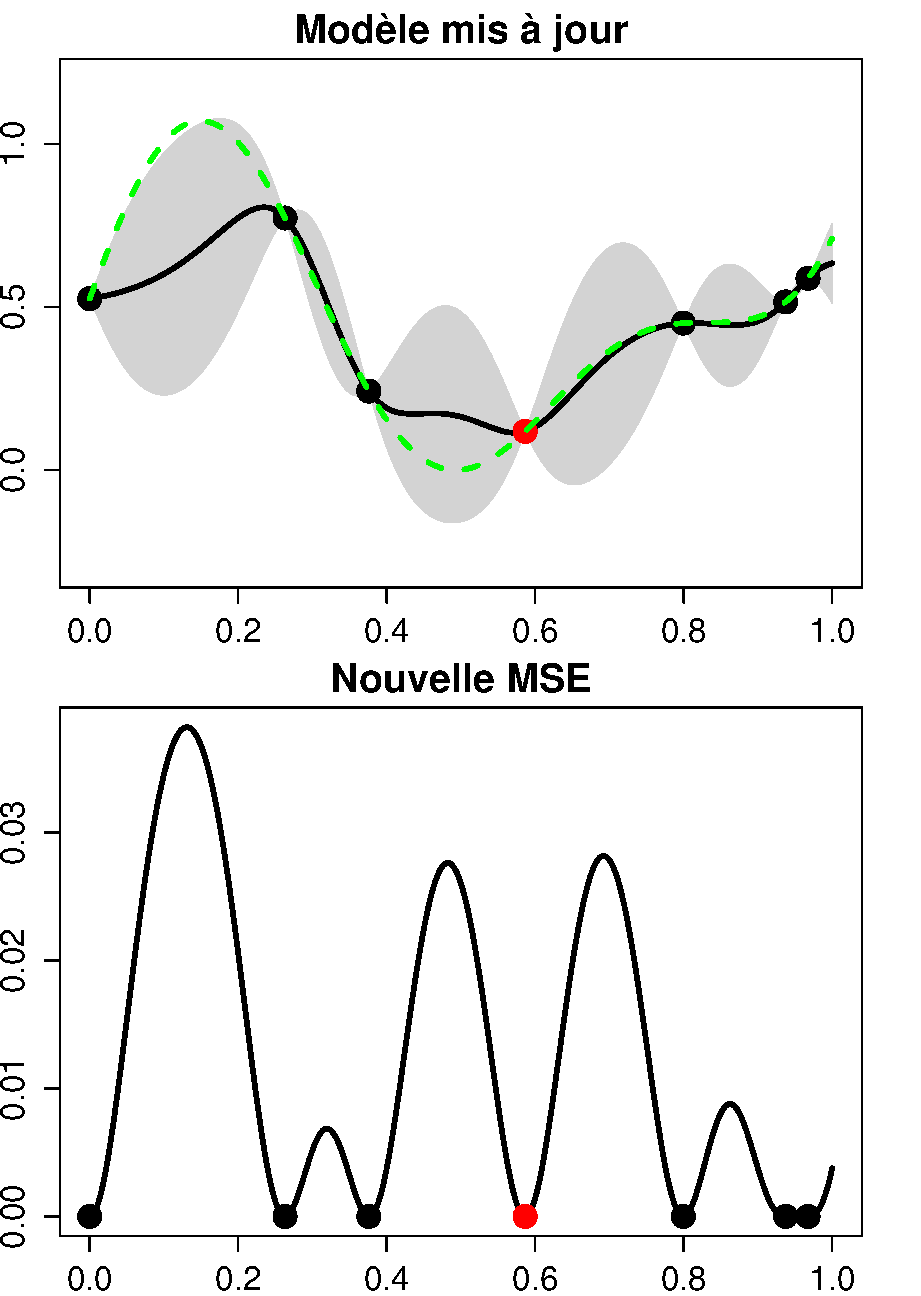
\includegraphics[width=.49\textwidth]{autres/MSE3.pdf}
\end{figure}
\end{frame}
%%%%%%%%%%%%%%%%%%%%%%%%%%%%%%%%%%%%%%%%%%%%%%%%%%%%%%%%%%%%%%%%%%%%%%%%%%%%%%%%%%%%%%%%%%%%%%%%%%
\begin{frame}{Exemple 2D : ``vraie'' fonction}
\begin{figure}
	\centering
	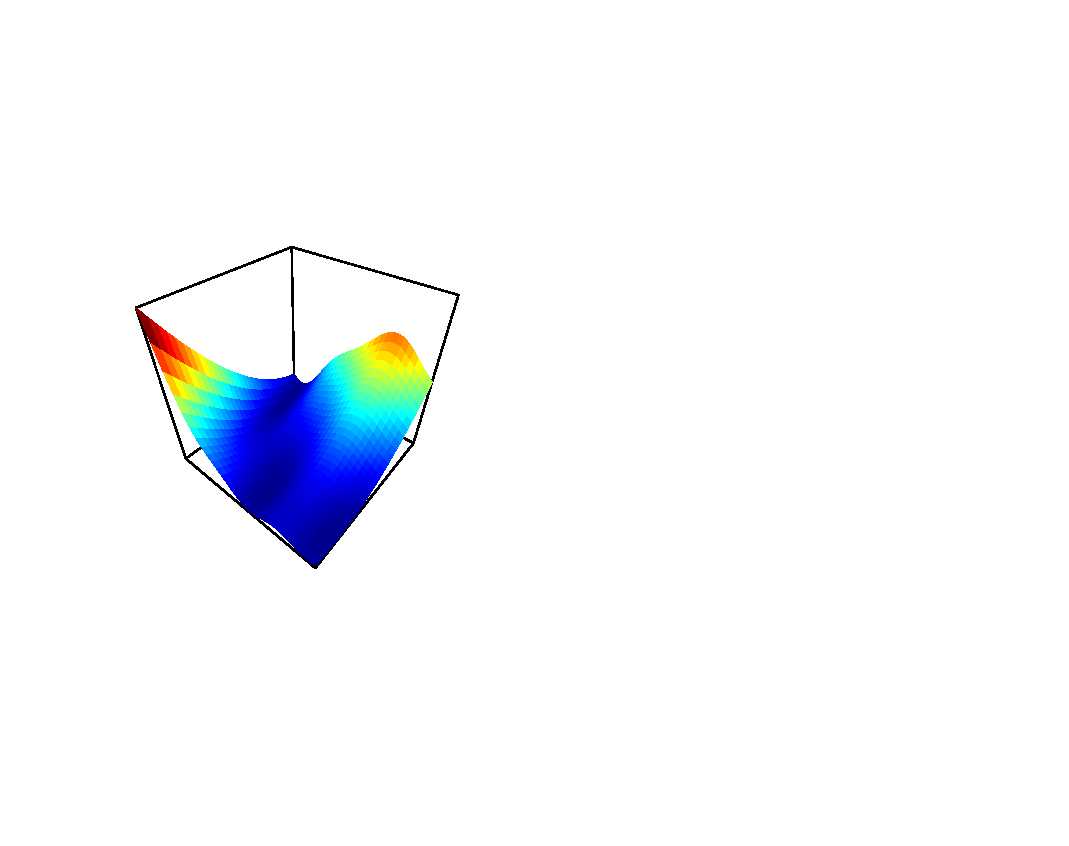
\includegraphics[trim=10mm 40mm 60mm 40mm,width=10cm, clip]{mse/initfun.pdf}
\end{figure}
\end{frame}
%%%%%%%%%%%%%%%%%%%%%%%%%%%%%%%%%%%%%%%%%%%%%%%%%%%%%%%%%%%%%%%%%%%%%%%%%%%%%%%%%%%%%%%%%%%%%%%%%%
\begin{frame}{Exemple 2D}
Plan de départ : 4 points
\begin{figure}
\hspace{5mm} Moyenne \hspace{50mm} Variance
	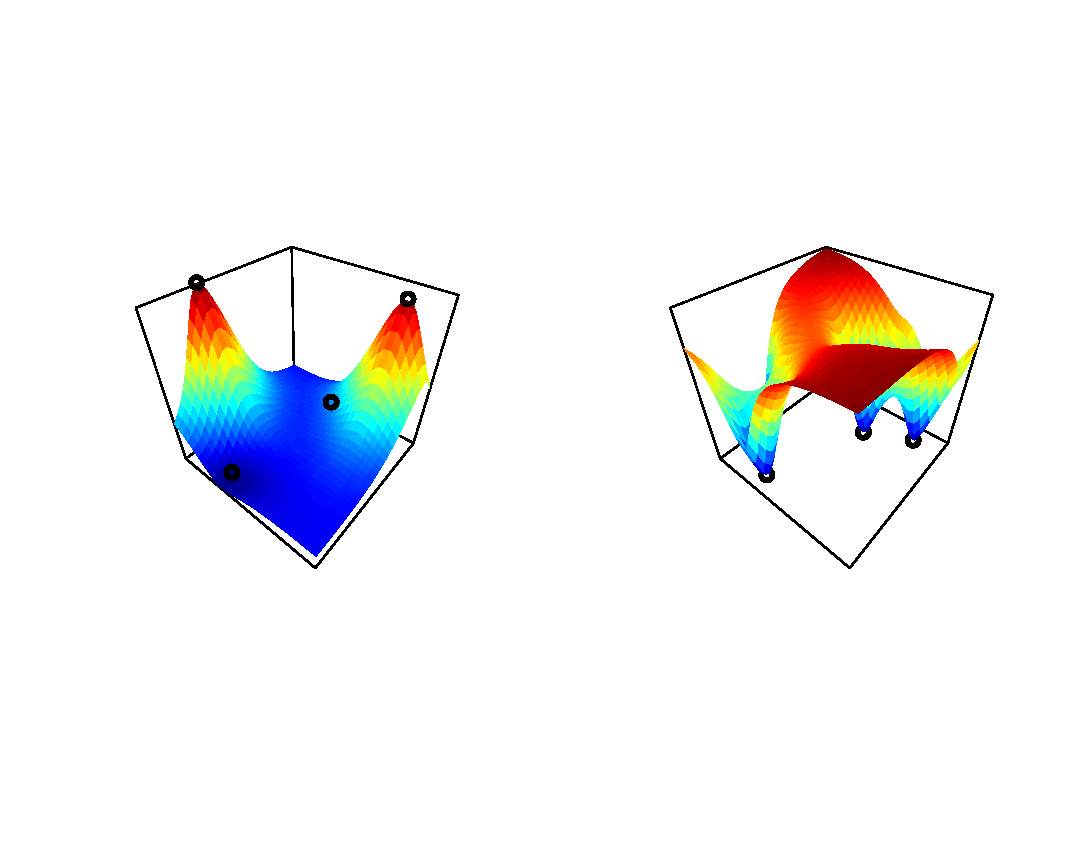
\includegraphics[trim=12mm 40mm 12mm 40mm,width=\textwidth, clip]{mse/maxMSE0.pdf}
\end{figure}
\end{frame}
%%%%%%%%%%%%%%%%%%%%%%%%%%%%%%%%%%%%%%%%%%%%%%%%%%%%%%%%%%%%%%%%%%%%%%%%%%%%%%%%%%%%%%%%%%%%%%%%%%
\begin{frame}[noframenumbering]{Exemple 2D}
5 points
\begin{figure}
\hspace{5mm} Moyenne \hspace{50mm} Variance
	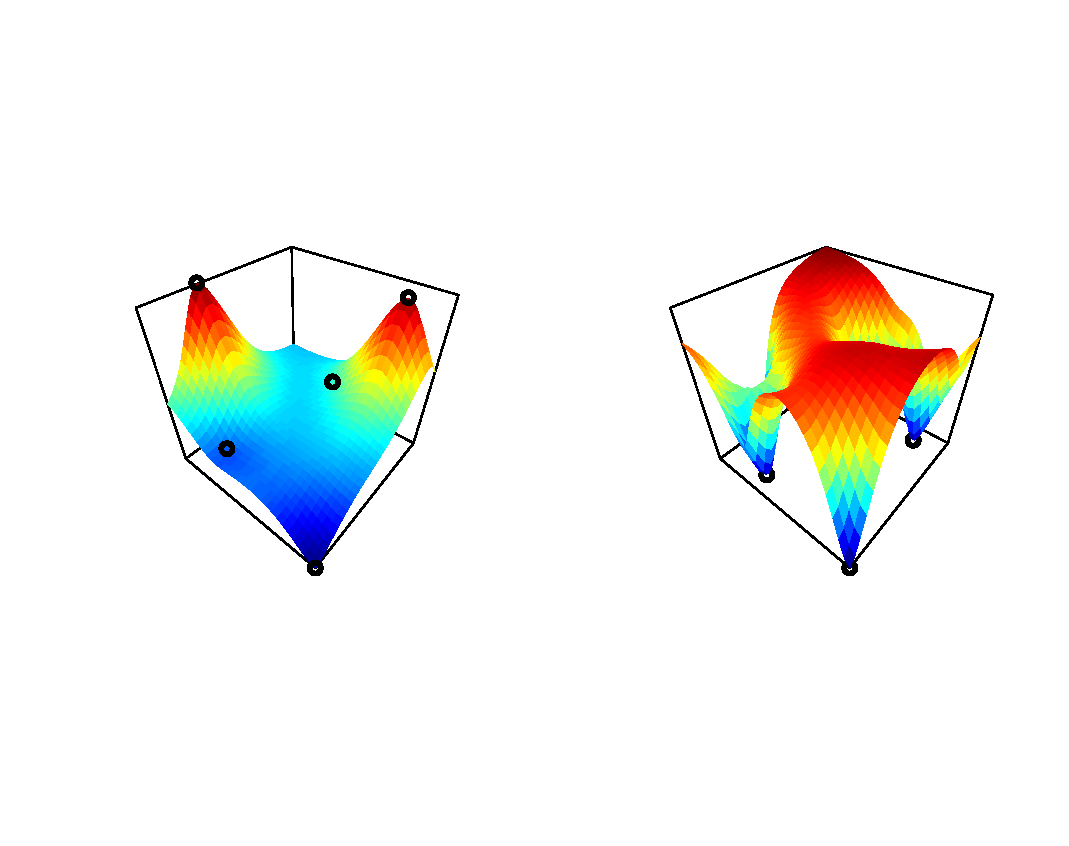
\includegraphics[trim=12mm 40mm 12mm 40mm,width=\textwidth, clip]{mse/maxMSE1.pdf}
\end{figure}
\end{frame}
%%%%%%%%%%%%%%%%%%%%%%%%%%%%%%%%%%%%%%%%%%%%%%%%%%%%%%%%%%%%%%%%%%%%%%%%%%%%%%%%%%%%%%%%%%%%%%%%%%
\begin{frame}[noframenumbering]{Exemple 2D}
6 points
\begin{figure}
\hspace{5mm} Moyenne \hspace{50mm} Variance
	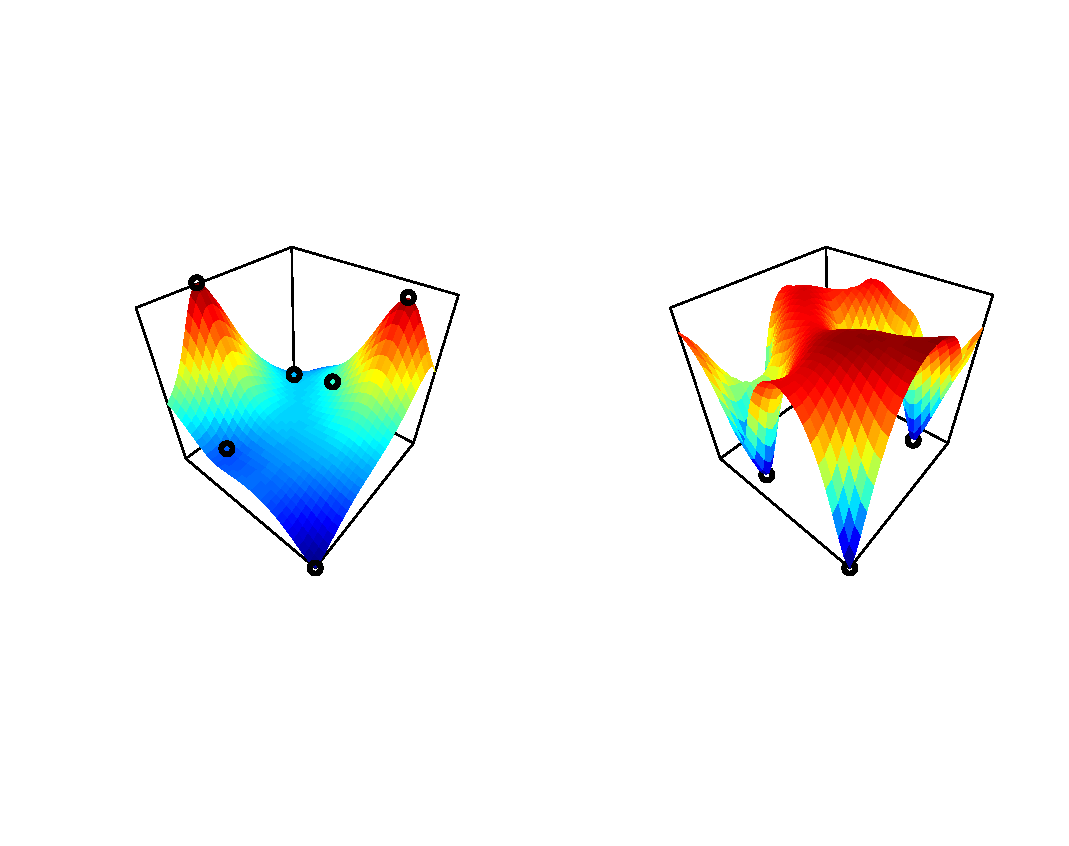
\includegraphics[trim=12mm 40mm 12mm 40mm,width=\textwidth, clip]{mse/maxMSE2.pdf}
\end{figure}
\end{frame}
%%%%%%%%%%%%%%%%%%%%%%%%%%%%%%%%%%%%%%%%%%%%%%%%%%%%%%%%%%%%%%%%%%%%%%%%%%%%%%%%%%%%%%%%%%%%%%%%%%
\begin{frame}[noframenumbering]{Exemple 2D}
7 points
\begin{figure}
\hspace{5mm} Moyenne \hspace{50mm} Variance
	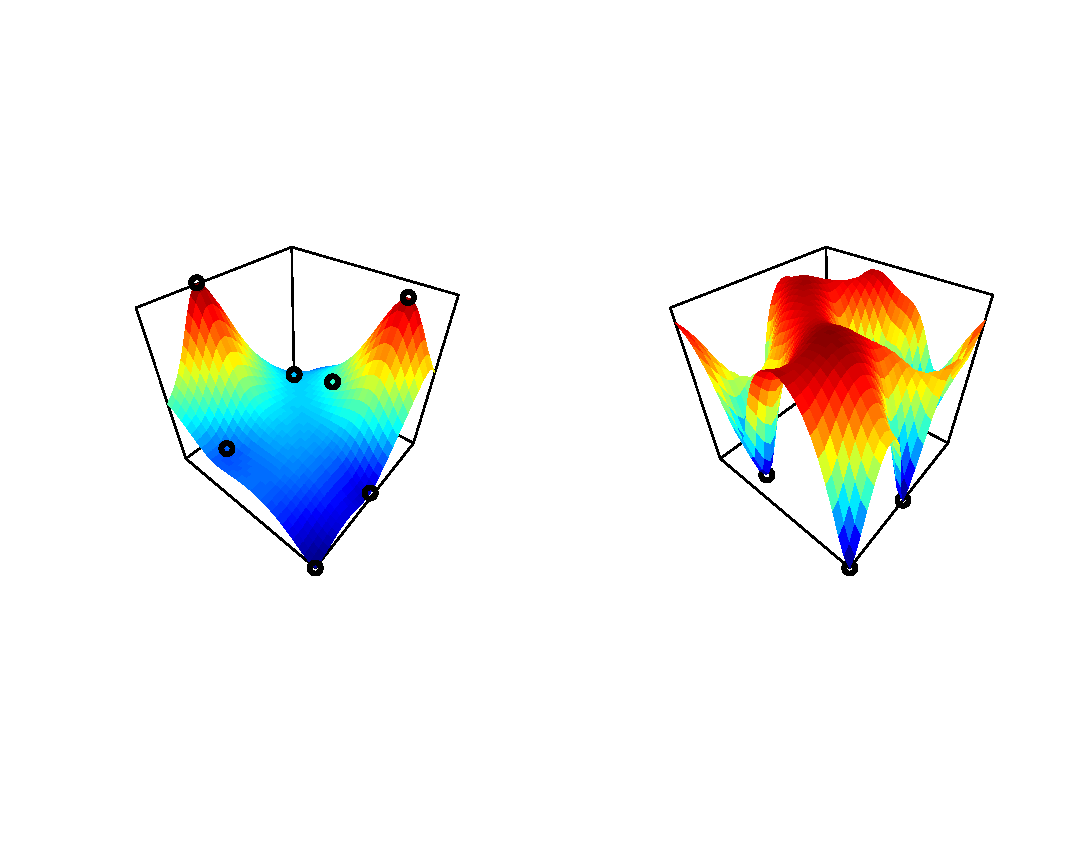
\includegraphics[trim=12mm 40mm 12mm 40mm,width=\textwidth, clip]{mse/maxMSE3.pdf}
\end{figure}
\end{frame}
%%%%%%%%%%%%%%%%%%%%%%%%%%%%%%%%%%%%%%%%%%%%%%%%%%%%%%%%%%%%%%%%%%%%%%%%%%%%%%%%%%%%%%%%%%%%%%%%%%
\begin{frame}[noframenumbering]{Exemple 2D}
8 points
\begin{figure}
\hspace{5mm} Moyenne \hspace{50mm} Variance
	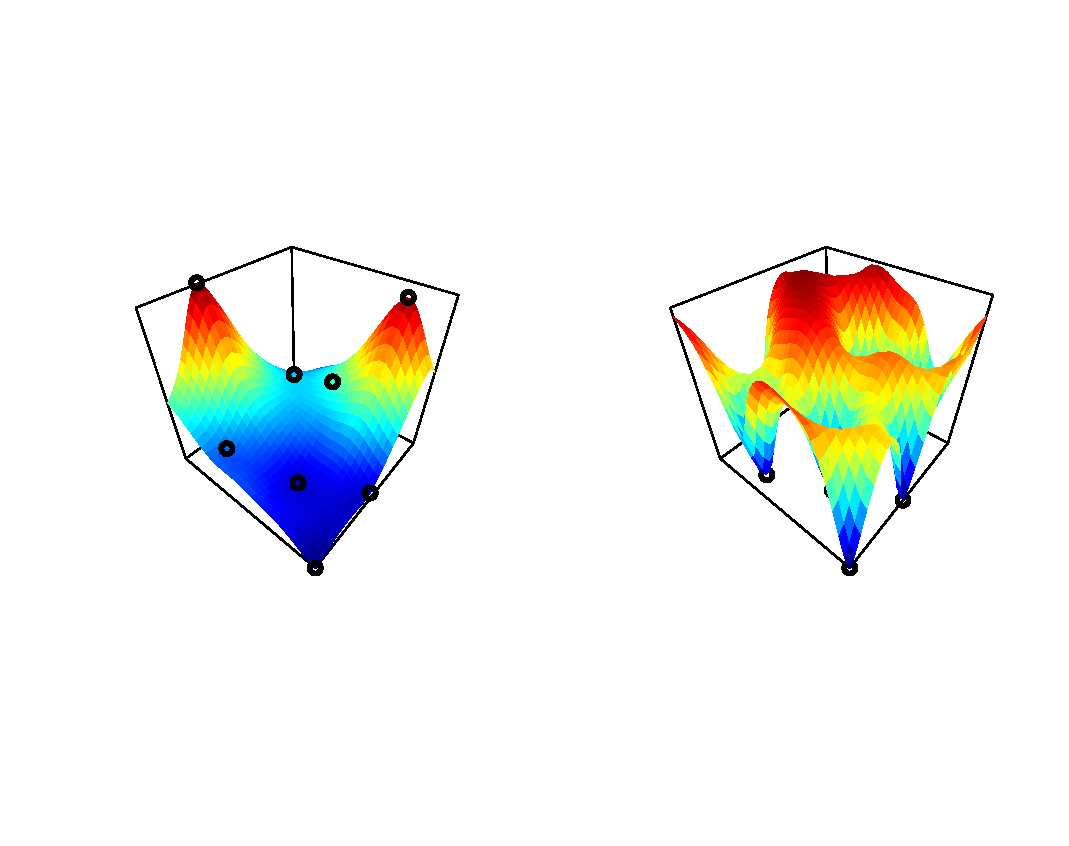
\includegraphics[trim=12mm 40mm 12mm 40mm,width=\textwidth, clip]{mse/maxMSE4.pdf}
\end{figure}
\end{frame}
%%%%%%%%%%%%%%%%%%%%%%%%%%%%%%%%%%%%%%%%%%%%%%%%%%%%%%%%%%%%%%%%%%%%%%%%%%%%%%%%%%%%%%%%%%%%%%%%%%
\begin{frame}[noframenumbering]{Exemple 2D}
14 points
\begin{figure}
\hspace{5mm} Moyenne \hspace{50mm} Variance
	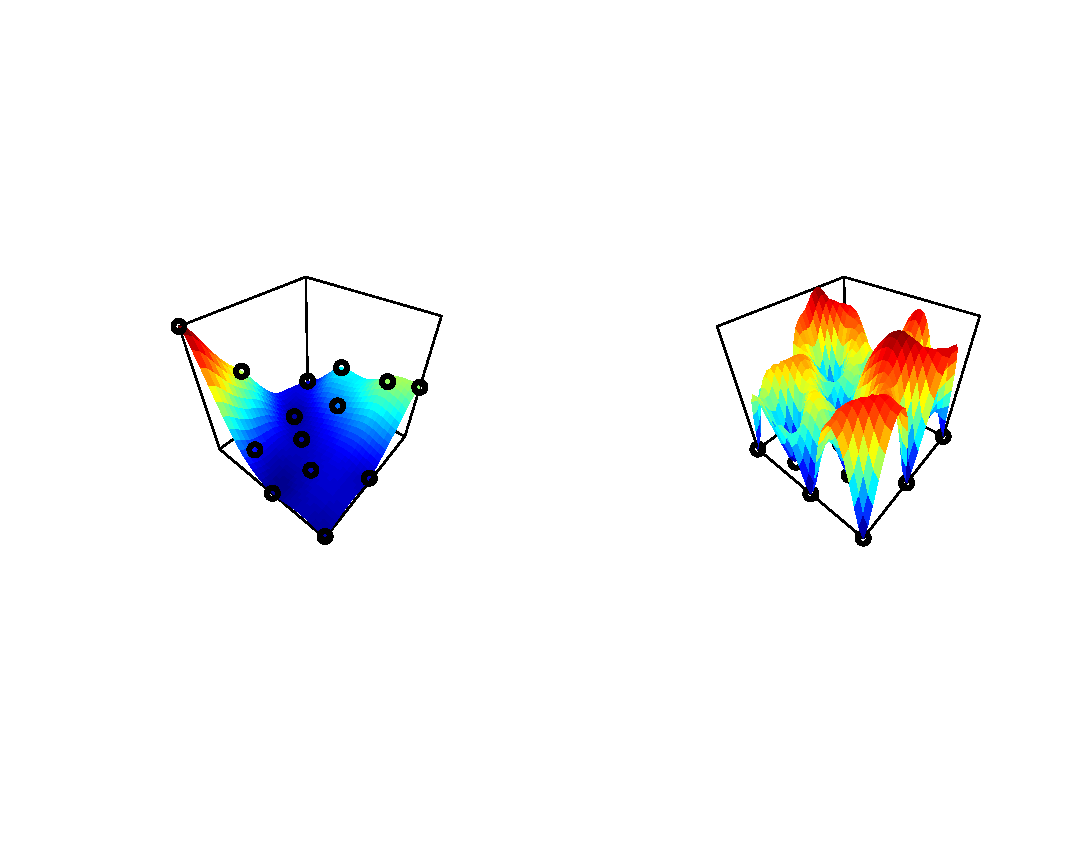
\includegraphics[trim=12mm 40mm 12mm 40mm,width=\textwidth, clip]{mse/maxMSE1414.pdf}
\end{figure}
\end{frame}
%%%%%%%%%%%%%%%%%%%%%%%%%%%%%%%%%%%%%%%%%%%%%%%%%%%%%%%%%%%%%%%%%%%%%%%%%%%%%%%%%%%%%%%%%%%%%%%%%%
\begin{frame}{Exemple 2D : plan final à 14 points}
\begin{itemize}
	\item Bon remplissage d'espace
	\item Tendance à échantillonner sur les bords
\end{itemize}

\begin{figure}
	\centering
	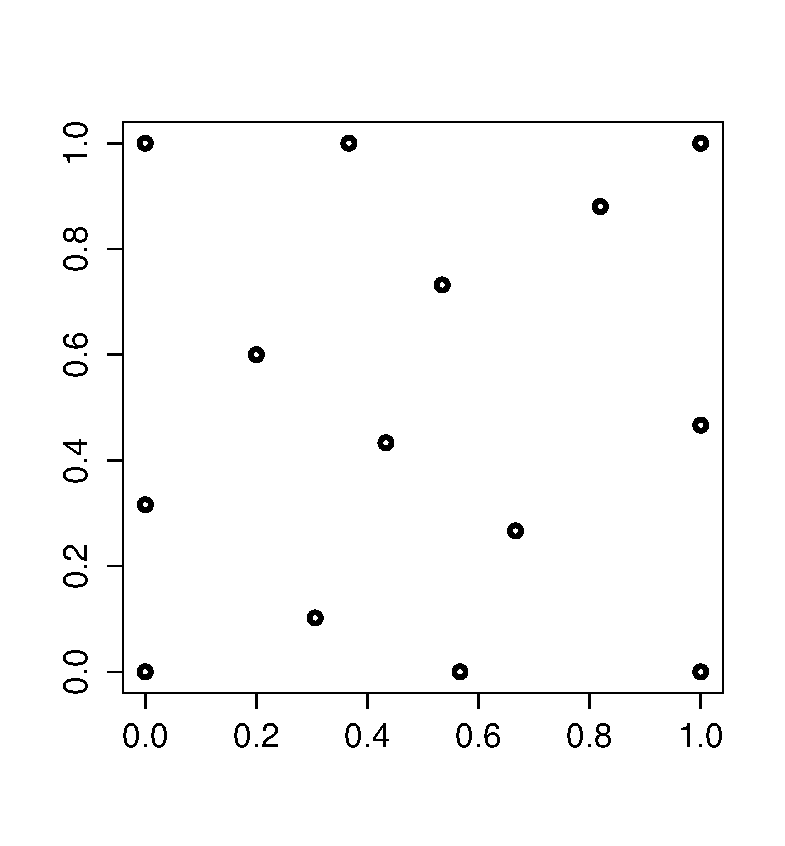
\includegraphics[trim=0mm 17mm 0mm 20mm,width=50mm, clip]{mse/maxMSE14.pdf}
\end{figure}

\begin{exampleblock}{Pour / contre}
 \begin{itemize}
	\item[$+$] Facile à mettre en place
	\item[$-$] Vraiment efficace ?
\end{itemize}
\end{exampleblock}
\end{frame}
%%%%%%%%%%%%%%%%%%%%%%%%%%%%%%%%%%%%%%%%%%%%%%%%%%%%%%%%%%%%%%%%%%%%%%%%%%%%%%%%%%%%%%%%%%%%%%%%%%
\begin{frame}{Maximum vs. moyenne de la MSE}
\begin{block}{Critère IMSE \textit{cf. cours de L. Pronzato}}
 $$IMSE = \int_D MSE(x)dx$$
 Erreur \textbf{moyenne} du modèle
\end{block}

\scriptsize{
 \begin{thebibliography}{1}
\beamertemplatearticlebibitems
     \bibitem{dace}
Sacks, Welch, Mitchell \& Wynn
  \newblock Design and analysis of computer experiments
  \newblock Statistical science, 409-423 (1989)
 \end{thebibliography}}

 \normalsize
\begin{exampleblock}{Utilisation dans une démarche séquentielle}
\begin{itemize}
 \item MSE : une valeur par point $\rightarrow$ recherche du maximum
 \item IMSE : valeur unique
\end{itemize}
On cherche le point qui diminue le plus le critère \textbf{si on l'ajoute au métamodèle}
\end{exampleblock}
\end{frame}
%%%%%%%%%%%%%%%%%%%%%%%%%%%%%%%%%%%%%%%%%%%%%%%%%%%%%%%%%%%%%%%%%%%%%%%%%%%%%%%%%%%%%%%%%%%%%%%%%
\begin{frame}{Comment évaluer le ``futur'' critère sans faire l'expérience ?}
 \begin{itemize}
  \item Retour sur la formule : $MSE(x) = \sigma^2 - k(x)^T \Sigma^{-1} k(x)$
  \item Ne dépend pas des valeurs observées $Z_S$
  \item On peut ajouter $x_{new}$ et choisir n'importe quelle valeur pour $Z(x_{new})$, l'IMSE reste la même.
 \end{itemize}
 
 \begin{block}{Principe}
Pour un point candidat $x_{new}$:
\begin{enumerate}
	\item On ajoute $x_{new}$ au plan d'expériences et une valeur quelconque aux observations
	\item On met à jour le métamodèle sans changer la covariance*
	\item On évalue le critère sur le nouveau modèle : $IMSE(x_{new})$
\end{enumerate}
On cherche $\mathbf{x}* = \arg \min_D IMSE(\mathbf{x})$.
\end{block}
\scriptsize{*ou, beaucoup plus efficace, on utilise des formules de mise à jour}
\end{frame}

%%%%%%%%%%%%%%%%%%%%%%%%%%%%%%%%%%%%%%%%%%%%%%%%%%%%%%%%%%%%%%%%%%%%%%%%%%%%%%%%%%%%%%%%%%%%%%%%%%
\begin{frame}{Illustration : maxMSE vs. minIMSE}
\begin{figure}
	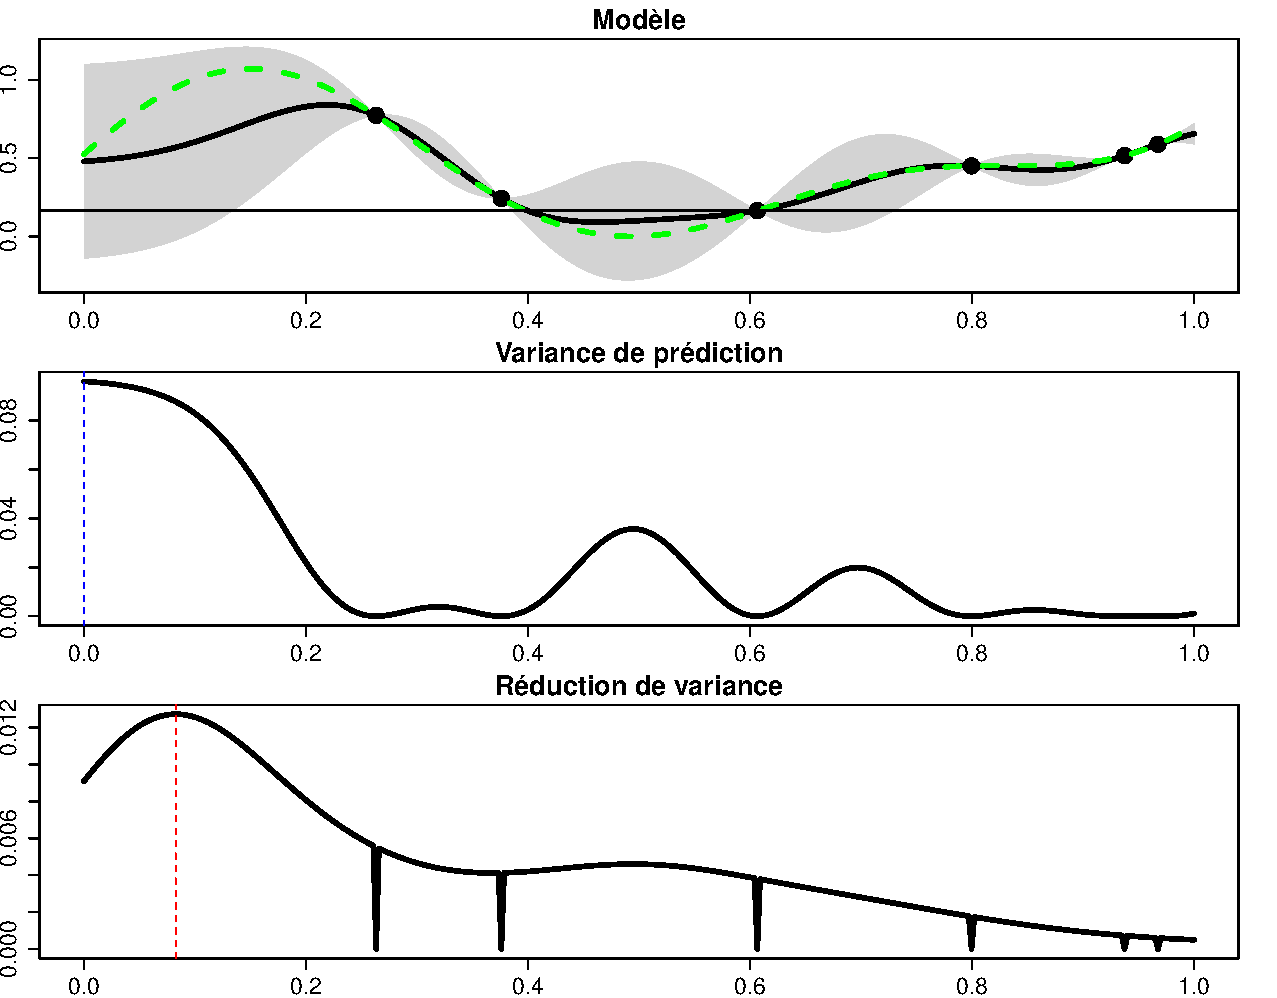
\includegraphics[width=.9\textwidth]{autres/maxMSEvsIMSE.pdf}
\end{figure}
\end{frame}
%%%%%%%%%%%%%%%%%%%%%%%%%%%%%%%%%%%%%%%%%%%%%%%%%%%%%%%%%%%%%%%%%%%%%%%%%%%%%%%%%%%%%%%%%%%%%%%%%%
\begin{frame}{Illustration : modèles mis à jour}
\begin{figure}
	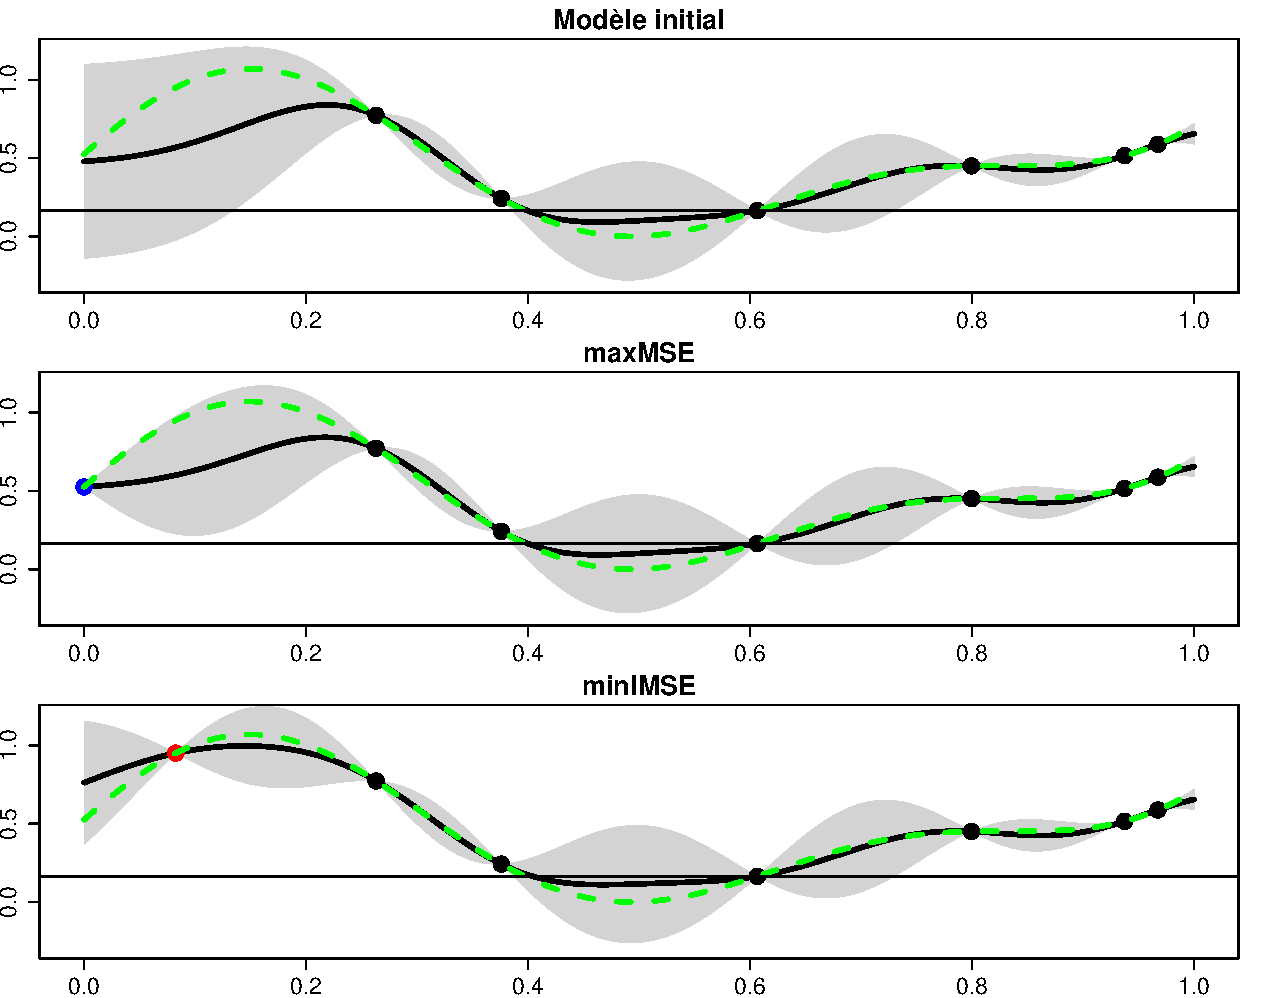
\includegraphics[width=.9\textwidth]{autres/maxMSEvsIMSE2.pdf}
\end{figure}
\end{frame}
%%%%%%%%%%%%%%%%%%%%%%%%%%%%%%%%%%%%%%%%%%%%%%%%%%%%%%%%%%%%%%%%%%%%%%%%%%%%%%%%%%%%%%%%%%%%%%%%%
\begin{frame}{Enrichissement séquentiel IMSE-optimal}
\begin{block}{Algorithme}
\begin{itemize}
 \item Même boucle que pour maxMSE
 \item Recherche du meilleur point $\Rightarrow$ boucle d'optimisation emboîtée
\end{itemize}
\end{block}

\begin{alertblock}{Critère sous forme intégrale}
Pas de formule analytique $\rightarrow$ intégration numérique
\end{alertblock}

\begin{exampleblock}{Parallélisation}
 On peut aussi chercher un ensemble de points IMSE-optimaux.
\end{exampleblock}

\end{frame}
%%%%%%%%%%%%%%%%%%%%%%%%%%%%%%%%%%%%%%%%%%%%%%%%%%%%%%%%%%%%%%%%%%%%%%%%%%%%%%%%%%%%%%%%%%%%%%%%%
\begin{frame}{Retour sur l'exemple 2D}
\begin{figure}
	\centering
	\hspace{5mm}maxMSE \hspace{35mm} minIMSE
	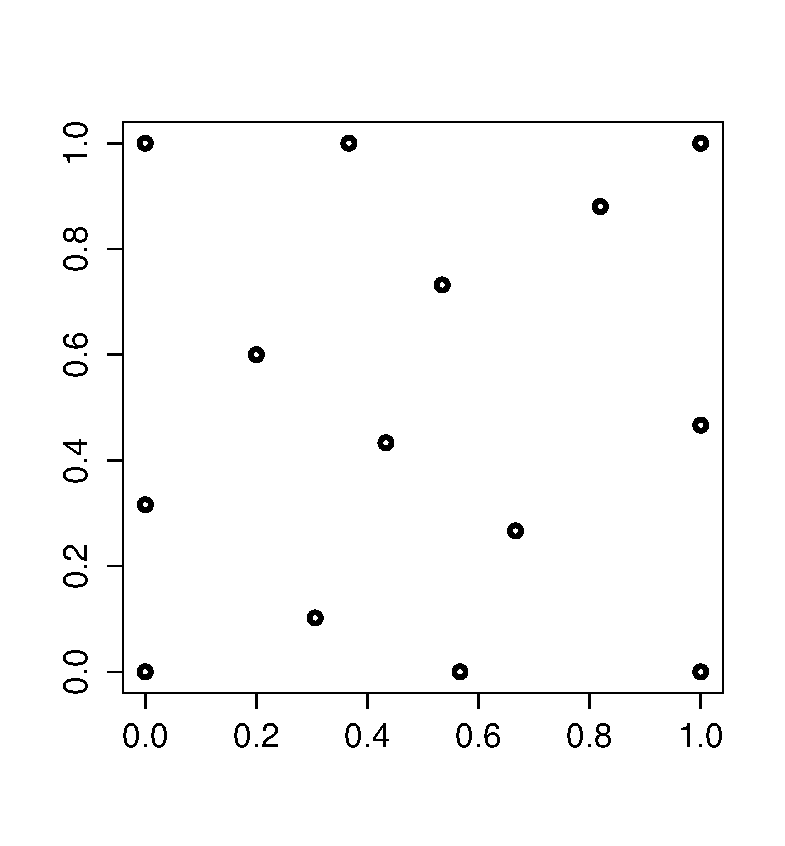
\includegraphics[trim=0mm 17mm 0mm 10mm,width=50mm, clip]{mse/maxMSE14.pdf}
	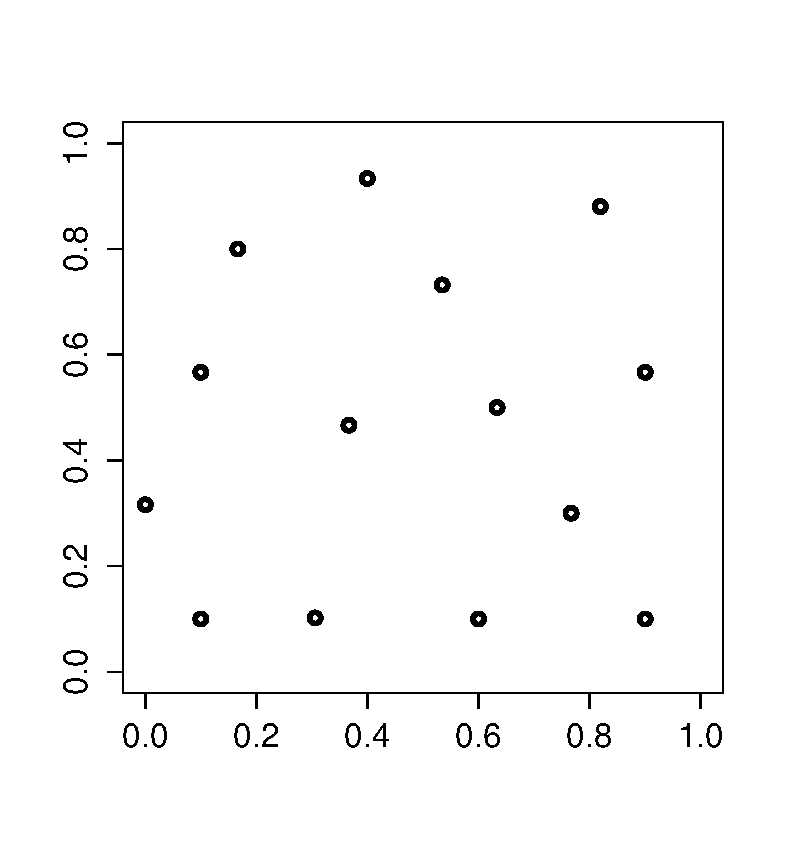
\includegraphics[trim=0mm 17mm 0mm 10mm,width=50mm, clip]{mse/minIMSE14.pdf}
\end{figure}
\end{frame}
%%%%%%%%%%%%%%%%%%%%%%%%%%%%%%%%%%%%%%%%%%%%%%%%%%%%%%%%%%%%%%%%%%%%%%%%%%%%%%%%%%%%%%%%%%%%%%%%%
\begin{frame}{Quelle stratégie choisir ?}
\begin{block}{minIMSE}
 \begin{itemize}
  \item[$+$] Correspond au but poursuivi
  \item[$+$] Pas d'effet de bord
  \item[$-$] Complexe : intégration numérique + mise à jour du modèle
  \item[$-$] Coûteux à évaluer  
 \end{itemize}
\end{block}

\begin{exampleblock}{maxMSE}
Exactement l'inverse !
\end{exampleblock}

$\Rightarrow$ Le choix dépend essentiellement du budget de calcul et de la dimension.

\end{frame}
%%%%%%%%%%%%%%%%%%%%%%%%%%%%%%%%%%%%%%%%%%%%%%%%%%%%%%%%%%%%%%%%%%%%%%%%%%%%%%%%%%%%%%%%%%%%%%%%%%